\documentclass[a4paper,10pt]{article}
\usepackage{epsfig}
\usepackage{latexsym}
\usepackage{graphicx}
\usepackage{amsfonts}
\usepackage{amsmath}
\usepackage{xcolor}

%-----------------------------------------
% Pour accepter les lettres accentuees de clavier azerty
% sans les \'e (utile) pour tapper directement en azerty 
% et ou faire passer aspell -c --lang=fr bidon.tex
%\usepackage[latin1]{inputenc}
%------------------------------------------

%\topmargin=-3cm
\topmargin=-1cm
\oddsidemargin=-1cm
\evensidemargin=-1cm
\textwidth=17cm
%\textheight=27cm
\textheight=25cm
\raggedbottom
\sloppy

\definecolor{Blue}{rgb}{0.,0.,1.}
\definecolor{LightSkyBlue}{rgb}{0.691,0.827,1.}
\definecolor{Red}{rgb}{1.,0.,0.}
\definecolor{Green}{rgb}{0.,1.,0.}
\definecolor{Purple}{rgb}{0.5, 0., 0.5}
\definecolor{Try}{rgb}{0.15,0.,1}
\definecolor{Black}{rgb}{0., 0., 0.}

\title{NIKA Polarization Leakage Correction applied to 3C273}
\author{N.~Ponthieu, A. Ritacco}

\begin{document}
\maketitle

\abstract{We apply a specific deconvolution/convolution technique to correct for
  the observed $I$ to $Q$ and $U$ leakage observed in NIKA data.}

\section{Introduction}

Immediately after the first polarized light of NIKA in September 2014,
observations of Uranus in polarization mode showed non zero $Q$ and $U$ signals
although Uranus has an unpolarized emission in our bands. This has been
confirmed by repeated observations during February 2015
(cf. Fig.~\ref{fig:uranus}).

%% \begin{figure}
%% \begin{center}
%% \includegraphics[clip, angle=0, scale = 0.5]{uranus_radec.png}
%% \caption{
%% Maps of $I$, $Q$ and $U$ of Uranus. $Q$ and $U$ are definitely non zero. This indicates a
%% systematic leakage from total power into Q and U at the $\sim 3\%$ level.}
%% \label{fig:uranus}
%% \end{center}
%% \end{figure}

The exact cause of this systematic effect remains unknown and while trying to
understand it, especially in preparation of NIKA2, we have been working on how
to correct for it. To first order, this is a leakage of total power into
polarization, and in this work, we'll limit ourselves to this description.

\section{Modelling}

In this work, we'll consider that each measure is the sum of the expected
measure, as seen by the integrated instrument with a ``perfect'' (mind the
quotes !) beam, and of the spurious leakage term that we want to correct
for. Observations of Uranus at various elevation have shown that the leakage is
fixed in Nasmyth coordinates.

Let's call $m$ the instantaneous measure of a kid and denote by a superscript $^N$
the Nasmyth coordinates, we have:

\begin{equation}
m = B_I * (I^N_0 + Q^N_0\cos2\alpha + U^N_0\sin2\alpha) + L_{IQ}*I^N_0\cos2\alpha +
L_{IU} * I^N_0\sin2\alpha + {\rm noise}
\end{equation}

where $\alpha$ accounts for the HWP angle and sky coordinates rotation and $B$ denotes
the instrumental beam. $L_{IX}$ the effective beam of the leakage. Uranus can
be considered as a point source compared to NIKA's FWHM. The polarized
observations of Uranus, once projected in Nasmyth
coordinates are then exactly the point spread functions or beams $L_{IQ}$ and
$L_{IU}$.

Our algorithm is thus:
\begin{enumerate}
\item Build a map of $I$, $Q$ and $U$ of the observed source in R.A. and
  Dec. This map can be the combination of multiple scans to have the best signal
  to noise.
\item Rotate this map in Nasmyth coordinates to obtain $I_N$, $Q_N$ and $U_N$.
\item Deconvolve $I_N$ from the instrumental beam to have an estimate of
  $\hat{I}_0$ of the true intensity.
\item Use Uranus Nasmyth maps of $Q$ and $U$ as $L_{IQ}$ and $L_{IU}$ to
  convolve $\hat{I}_0$ and produce maps of the expected leakage.
\item Scan these maps to produce timelines and subtract these timelines from the
  original data
\item Projected these corrected data onto final maps.
\end{enumerate}

The deconvolution/convolution steps 3 and 4 are performed at the same time in Fourier
space:

\begin{equation}
(I^N_0*L_{IQ})(k) = I^N_0(k) \times L_{IQ}(k) \simeq I^N(k)/B_I(k)\times L_{IQ}(k)
\end{equation}

The ratio $L_{IQ}(k)/B_I(k)$ is tapered so that the division by decreasing terms
of $B_I(k)$ when $k$ increases is counterbalanced by the deaming of
$L_{IQ}(k)$. The exact range of this tapering still needs to be optimized.


\section{In practice}

Let's take $3C273$ as a test case.

\subsection{Recentering}

\begin{figure}
\begin{center}
\includegraphics[clip, angle=0, scale = 0.2]{figures/ptg_offset_20150217s45.eps}
\includegraphics[clip, angle=0, scale = 0.2]{figures/ptg_offset_20150217s46.eps}
\includegraphics[clip, angle=0, scale = 0.2]{figures/ptg_offset_20150217s47.eps}
\includegraphics[clip, angle=0, scale = 0.2]{figures/ptg_offset_20150217s48.eps}
\caption{Intensity maps of $3C273$ before pointing corrections. The quasar is
  off-centered y a few arcseconds.}
\label{fig:ptg_offsets}
\end{center}
\end{figure}

We first build maps of the quasar with no correction to determine the pointing
offsets (Fig.~\ref{fig:ptg_offsets}). Indeed, the pointing corrections applied during observations do not
prevent from all the pointin shifts accross time, and it is important to account
for this before coadding maps to avoid bluring the final images. The pointing
corrections to apply to a given scan are stored and do not need to be
re-estimated.

\subsection{Leakage correction}

\begin{figure}
\begin{center}
\includegraphics[clip, angle=0, scale = 0.4]{figures/Radec2nasmyth_vs_lkg_correction_20150217s45.eps}
\caption{\emph{Top:} Uncorrected data maps of $Q$ and $U$ in Nasmyth
  coordinates. \emph{Bottom:} Estimates of the leakage terms. One can see the
  resemblance of the two. The apparent ringing comes from the sharp edge
  tapering of the kernels and should easily be improved in the near future.}
\label{fig:data_vs_lkg}
\end{center}
\end{figure}

\begin{figure}
\begin{center}
\includegraphics[clip, angle=0, scale = 0.3]{figures/I_3C273_1mm_uncorr.eps}
\includegraphics[clip, angle=0, scale = 0.3]{figures/Q_3C273_1mm_uncorr.eps}
\includegraphics[clip, angle=0, scale = 0.3]{figures/U_3C273_1mm_uncorr.eps}
\includegraphics[clip, angle=0, scale = 0.3]{figures/I_3C273_1mm_corr.eps}
\includegraphics[clip, angle=0, scale = 0.3]{figures/Q_3C273_1mm_corr.eps}
\includegraphics[clip, angle=0, scale = 0.3]{figures/U_3C273_1mm_corr.eps}
\caption{\emph{Top:} Uncorred data maps of $I$, $Q$ and $U$ in R.~A.~and Dec. at
  1mm. \emph{Bottom:} Data maps corrected from the leakage term. The dipolar
  pattern, more visible in $Q$ has disappeared, leaving at the center, the
  polarized signal of the quasar. This is clearer at 2mm on Fig.~\ref{fig:final_results_2mm}.}
\label{fig:final_results_1mm}
\end{center}
\end{figure}

\begin{figure}
\begin{center}
\includegraphics[clip, angle=0, scale = 0.3]{figures/I_3C273_2mm_uncorr.eps}
\includegraphics[clip, angle=0, scale = 0.3]{figures/Q_3C273_2mm_uncorr.eps}
\includegraphics[clip, angle=0, scale = 0.3]{figures/U_3C273_2mm_uncorr.eps}
\includegraphics[clip, angle=0, scale = 0.3]{figures/I_3C273_2mm_corr.eps}
\includegraphics[clip, angle=0, scale = 0.3]{figures/Q_3C273_2mm_corr.eps}
\includegraphics[clip, angle=0, scale = 0.3]{figures/U_3C273_2mm_corr.eps}
\caption{\emph{Top:} Uncorred data maps of $I$, $Q$ and $U$ in R.~A.~and Dec. at
  2mm. \emph{Bottom:} Data maps corrected from the leakage term. The dipolar
  pattern in $Q$ and $U$ has disappeared, leaving at the center, the
  polarized signal of the quasar.}
\label{fig:final_results_2mm}
\end{center}
\end{figure}

A first estimate of $I$, $Q$ and $U$ maps in R.A. and Dec is obtained and used
as input signal for the correction. Actually, only $I$ is
used. These maps are then rotated into Nasmyth coordinates (Fig.~\ref{fig:radec2nasmyth})

The itensity map in Nasmyth coordinates is then deconvolved by the intensity
beam and convolved by the leakage kernels. The produced leakage maps can then be
compared to the yet uncorrected data maps in Nasmyth coordinates (Fig.~\ref{fig:data_vs_lkg}).

The leakage maps are then scanned according to each kid pointing to produce
timelines that are subtracted from the input $Q$ and $U$ TOI's. We then proceed
to the final projection. A comparison, of the maps with and without correction
is presented on Figs.~\ref{fig:final_results_1mm} and \ref{fig:final_results_2mm}.


\section{Next}
Many parameters, such as the apodization of the leakage kernels, the maximum
frequency that we tolerate in this deconvolution/convolution, the noise
behaviour (increase ? correlation ?) remain to be characterized and
optimized. This must also be applied and characterized on extended sources such
as the Crab. For now, the maximum $k$ considered in the deconvolution is
suitable for point sources, but not for the Crab, although we checked that the
pipeline did run correctly on the Crab scans.

%----------------------------------------------------------------------------------------
\begin{thebibliography}{}
\end{thebibliography}

\end{document}
